\documentclass{llncs}  % from http://www.springer.de/comp/lncs/authors.html
\pagestyle{headings}   % turn on page numbers for the reviewers

\usepackage{times}
\usepackage[dvips]{graphicx}
\usepackage{myZstan}
\usepackage{alltt}
\newcommand{\Zeta}{Zeta}

% \TODO{Write a longer version of this paper which includes more of Ian's
%   comparison of predicate and expression structures and rationale
%   for their XML format.}
% \TODO{Make font in Fig. 7 smaller}
% \TODO{Mention that The ``permissive, egalitarian style of mark-up'' might
% be recognised by some as the literate style promoted by Knuth in his web
% systems.}  

% Temporary, until I get the Zstan package.
% \usepackage{oz}
% \newcommand{\AFont}[1]{\texttt{#1}}
% \newcommand{\CADiZ}{CADIZ}
% \newcommand{\ASpecification}{Specification}
% \newcommand{\ASection}{Section}
% \newcommand{\AParagraph}{Paragraph}
% \newcommand{\APredicate}{Predicate}
% \newcommand{\AExpression}{Expression}
% \newcommand{\TNAME}{TNAME}
% \newcommand{\ASectTypeEnv}{SectTypeEnv}
% \newcommand{\ASignature}{Signature}
% \newcommand{\CFreetype}{Freetype}
% \newcommand{\CBranch}{Branch}
% \newcommand{\CPrec}{Prec}
% \newcommand{\CAssoc}{Assoc}
% \newcommand{\DTanonspec}{\par TODO: show DTanonspec here \par}
% \newcommand{\DTschemadef}{\par TODO: show DTschemadef here \par}
% \newcommand{\DTgenschemadef}{\par TODO: show DTgenschemadef here \par}
% \newcommand{\DThorizdef}{\par TODO: show DThorizdef here \par}
% \newcommand{\DTgenhorizdef}{\par TODO: show DTgenhorizdef here \par}
 
\newcommand{\TODO}[1]{\textbf{TODO: #1}}   % For draft version
% \newcommand{\TODO}[1]{}    % For final version

\title{ZML: XML Support for Standard Z}
\author{Mark Utting\inst{1} 
        \and Ian Toyn\inst{2}
        \and Jing SUN\inst{4}
        \and Andrew Martin\inst{3}
        \and Jin Song DONG\inst{4}
        \and Nicholas Daley\inst{1}
        \and David Currie\inst{5}
}
\institute{The University of Waikato, Hamilton, NZ\\
        \email{\{marku,ntd1\}@cs.waikato.ac.nz}
  \and  The University of York\\
        Email: \texttt{ian@cs.york.ac.uk}
  \and  Oxford University\\
        Email: \texttt{Andrew.Martin@comlab.ox.ac.uk}
  \and  The National University of Singapore \\
        Email: \texttt{\{sunjing,dongjs\}@comp.nus.edu.sg}
  \and  IBM UK Labs, Hursley Park, Winchester, Hants, UK \\
        Email: \texttt{david\_currie@uk.ibm.com} 
}

\begin{document}
\maketitle

\begin{abstract}
  This paper proposes an XML format for standard Z.
  We describe several earlier XML proposals for Z,
  the problems and issues that arose, and the rationales
  behind our new proposal.
  The new proposal is based upon a comparison of various existing Z
  annotated syntaxes, to ensure that the mark-up will be widely usable.
  This XML format is expected to become a central feature of
  the CZT (Community Z Tools) initiative.
\end{abstract}

\section{Why an XML format for Z?}

The publication during 2002 of the ISO Z Standard~\cite{ISOZ}
represents a significant milestone for the development and
interoperability of Z tools.  It has established what notation should be
exchanged, but not necessarily how.  Technology has advanced during the
development of the standard, so it now seems most natural for tools
to interact using an XML mark-up \cite{XML}.

This paper describes such a mark-up, intended to be a development of the
Standard's work, as a contribution to the Community Z Tools\footnote{See
  \url{http://web.comlab.ox.ac.uk/oucl/work/andrew.martin/CZT}.}  (CZT)
initiative.  CZT has been proposed in response to the observation that
many interesting Z tools have been developed, but few have built large
user communities, and many have found it necessary to invest
disproportionately large amounts of effort in the relatively mundane
activities of parser and pretty-printer development.  The initiative aims
to define interfaces and interchange facilities (and later, code
libraries) which Z tool developers can draw on in an open-source spirit,
with the aim both of promoting interoperability and of relieving those
wishing to develop novel tools for visualisation, animation, refinement,
proof, and so on, from the need to invest effort in the user interface
code.

XML is a development, like HTML, from the SGML~\cite{SGML86}.  Early drafts
of the Z Standard included an SGML mark-up, but it was found hard to
maintain. XML now enjoys a much wider take-up than SGML, having quickly
become a new standard for structured information interchange between tools.

Without such a mark-up, Standard Z allows specifications to be exchanged
using Unicode (UCS\cite{ISO10646-1,ISO10646-2}).
However, this representation is suitable only
for interchanging raw (unparsed) Z specifications, without annotation.
Tools (and sometimes authors) benefit from being able to annotate terms
with type information, anticipated usage and refinement targets, free-form
comments, and so on.   A particular presentation (on paper, on screen, or
within program data structures) may make use of some of these annotations
and discard others.  An XML format facilitates the inclusion of such
annotations, with as little or as much structure as is appropriate.  In
the longer term, when this use of XML reaches greater maturity, we would
expect the format described here to become part of the ISO Z Standard.


\subsection{Requirements of a Z interchange mark-up}\label{injectivity}

We have three requirements for an XML mark-up for Z.
 
\paragraph{Annotations.}
The already mentioned annotations should be accommodated
in the interchange mark-up wherever tools wish to put them.
The forms of individual annotations should not be constrained.
There should be some pre-defined annotations for types and for
source-file locations (so that error messages can refer to the
source of an error), but it should also be possible for tools
to define additional annotations.  Tools that do not understand
such annotations should simply ignore them.

\paragraph{Injectivity.}
The concrete syntax of Z provides different ways of writing the 
same things.  For example, a boxed schema paragraph
may be written in an equivalent definitional form, without the box.
After a specification has been transferred between tools, the user wants
to be reassured as much as possible (by avoiding unexpected changes 
of presentation) that their specification document has not been changed.
Consequently, the interchange mark-up for Z should capture
sufficient information from the concrete representation 
to be able to resurrect the same concrete phrases
(though not necessarily the same layout).
In other words, we want the conversion of a textual Z specification into 
XML format to be one-to-one (injective), so that the concrete 
representation before and after interchange, ignoring annotations,
remains recognisably the same.
For the schema paragraph example, this means keeping a note of whether 
or not the boxed representation is used. 
In this paper, we avoid using the traditional term \textit{abstract syntax}
because of this avoidance of loss of information from the concrete form.

\paragraph{Commonality.}
Conversely, for reasons of simplicity and demonstrable soundness, 
tools should need to deal with as few cases as possible.  This implies
that we should merge equivalent concrete constructs whenever possible
(the Z standard has a large number of transformation rules that do
exactly this).
For example, a tool might offer to display the signature 
of a schema paragraph regardless of whether or not it is boxed.
This is easier if a common \textit{annotated syntax} is used
for both of the concrete representations of the schema paragraph.
Interchange will be eased if the mark-up is based on an annotated syntax
that identifies similar commonalities to those exploited by tools.
In this paper, we use two approaches to merging constructs while preserving
injectivity:
\begin{enumerate}
\item using a common XML tag for two similar constructs, but adding
  attributes to distinguish between the constructs; 
\item using distinct XML tags and adding a common type hierarchy above
them to reflect their commonality.
\end{enumerate}
The second approach has an additional advantage: the type hierarchy of
commonality is similar to a typical inheritance hierarchy in
object-oriented programs, which makes it easier to map between the XML
structure and Java or C++ classes.  This is useful, because one of the
CZT aims is to develop a Java library for building Z tools.

\vspace{1.5ex}

The annotated syntaxes used within existing tools have already
addressed these issues of annotations, injectivity and commonalities.
The annotated syntax used within Standard Z addresses some of these issues.
An interchange mark-up for Z will be easier for a tool to use
if the mark-up is similar to the tool's own annotated syntax,
but there is considerable variation between existing tools. 

This paper compares some existing annotated syntaxes and describes an
XML mark-up based on their common features or best features. 
We aim to define a mark-up that will be usable not only by proposed CZT
developments but also by developments of existing tools.  Hence,
we are interested to receive feedback from other tool builders.


\subsection{Specifying the XML structure: DTD or XML Schema?}

There are many different ways in which Z specifications could be
expressed in XML.  
To specify exactly which structures of XML we propose to
use, and the well-formedness conditions on those structures, we need to
specify a particular subset of XML.
Such a specification is typically written in either of two languages:
as a \textit{Document Type Definition} (DTD), or as an \textit{XML
  Schema}.  The provision of such a specification allows a
\textit{validating parser} to perform more accurate well-formedness
checking, and is useful to toolbuilders for defining what tools should be
able to interchange.
% The simple syntax of XML allows tools to communicate
% without a DTD or XML Schema (using a \textit{non-validating parser}).

The DTD notation is older and simpler than the XML Schema notation, and
more human-readable, but the XML Schema language allows better
specification of the data types of elements than the DTD language.  XML
Schema has many built-in datatypes such as string, integer, boolean, float,
date, time and so on, and provides mechanisms to constrain the allowable
content of an element or attribute, such as setting a valid range of values
or defining a regular expression to which the content must conform.  New
types can be defined from scratch or by constraining or extending an
existing type.  This allows hierarchies of complex types to be constructed.
Furthermore, XML Schemas are themselves written in XML.  This makes the
document descriptions more verbose, but also far more extensible than they
were in the original DTD syntax. Declarations can have richer and more
complex internal structures than declarations in DTDs. Thus XML Schemas can
be stored along with other XML documents in XML-oriented data stores,
referenced, and even styled, using tools like XLink, XPointer, and
XSLT\footnote{See \url{www.w3.org}.}. For our purposes, we prefer to use XML
schema notation, to obtain a tighter specification of the structure, and to
take advantage of XML tools, such as XSLT.


\section{Previous Work}

There were earlier attempts to define XML mark-ups for Z
\cite{Wordsworth99,Dong01} but these did not support the interchange of
annotations such as the types of expressions, and were based on an earlier
version of Z, described by Spivey~\cite{spivey:z-notation2}. 
For example, Z/EVES~\cite{saaltink:zeves-system} supports an XML mark-up
for communication between tools, based on Spivey Z.

Before ZB2002, Toyn wrote a DTD for Standard Z, influenced by the
abstract syntaxes of \CADiZ\ and \Zeta.  This DTD has heavily influenced our
proposal in this paper. 

For example, here is the top-level element declaration from that DTD:
\begin{small}
\begin{verbatim}
<!ELEMENT Z:Spec; (((Z:Sect;*), Z:SpecAnns;?) | Z:PCDATA)>
\end{verbatim}
\end{small}

This defines a Z specification to be either a sequence of sections
followed by an optional \emph{specification annotations} element, or a
\AFont{PCDATA} alternative, which is another element that is defined 
to contain just \verb!#PCDATA! (\textit{parsed character data}).
Every element in the DTD includes a \AFont{Z:PCDATA} alternative, so
that if one part of a specification contains an error, the whole
specification can still be passed between tools.  For example,
a fully-parsed specification might be passed to an editor, and after
editing is complete, the editor might pass it back with unchanged
portions still in parsed form, but the edited portions in \AFont{Z:PCDATA}
form. 

During 2002, David Currie validated the DTD, and Utting and Daley
manually derived a Java class hierarchy from it~\cite{daley:report02}.
During this process, we identified several difficulties with the
DTD structure:

\begin{enumerate}
\item The presence of an `unparsed' alternative for \emph{every} element
  allowed extremely fine-grained portions of the specification to be left
  unparsed, but dramatically complicated the Java class hierarchy.
  Basically, every element \verb!E! of the DTD had to be translated into
  \emph{three} Java classes: an abstract class \verb!E! and two concrete 
  subclasses, \verb!EParsed! and \verb!EUnparsed!, where \verb!EParsed!
  contained fields that matched the parsed structure and \verb!EUnparsed!
  contained just an unparsed string.  The real disadvantage of this was
  that every piece of Java code that accessed an \verb!E! object had to
  immediately check whether it was parsed or unparsed.  This issue was not
  specific to Java, but would affect processing in every language.
  
  To solve this problem, our new proposal in this paper limits the
  \emph{granularity} of the unparsed portions so that an entire paragraph
  (for example, one schema) is the smallest
  unparsed portion allowable.  This simplifies processing, because it means
  that only the top-level of processing needs to consider unparsed portions
  and once we see a parsed paragraph, we know that everything inside it
  will also be parsed.

\item Each element in the DTD has its own kind of annotation, as
  illustrated in the example above (\verb!SpecAnns!).  Each kind of
  annotation is given 
  a default definition in the DTD (expression annotations contain just a
  type, schema annotations contain a signature etc.), but can be
  overridden by providing an extended DTD that adds extra fields.
  However, because each kind of expression has its own kind of annotation,
  it is necessary to override all 23 kinds of expressions 
  to add a new annotation to expressions (or 7 kinds for predicates, 
  5 kinds for paragraphs, etc.).
  
  To solve this problem, and make it easier to add new kinds of
  annotations, we have changed to a more loosely-typed view of annotations
  that is similar to the annotations in \Zeta.  Each Z construct can contain
  a list of arbitrary annotations.  This
  means that a tool could attach an annotation to an inappropriate
  construct (such as putting a type annotation on a predicate), but such
  annotations do no harm and can simply be ignored.  On the other hand,
  there are many kinds of annotations (such as hyperlinks, source-code
  positions and comments), that we want to be able to attach to arbitrary
  constructs, and this is easier with these loosely-typed annotations.
  
\item In an object-oriented class hierarchy, it is possible to organise
  the hierarchy to reflect commonality, so that common fields and methods
  can be inherited.  This is more flexible than the DTD structure, which
  does not have any kind of inheritance.  This resulted in more differences
  between the DTD structure and our ideal Java class hierarchy than we
  would have liked. 

  Our new proposal solves this problem by using XML Schema to specify the
  structure of the Z mark-up.  XML Schema offers a rich set of (single)
  inheritance features between types, as well as a \emph{substitution
  group} facility which is similar to subtyping in object-oriented
  languages.  
\end{enumerate}


Also in 2002, at the National University of Singapore, Dong and Sun
developed a new version of their XML Schema, based more closely on
the annotated syntax structure of the Z standard.  This did not
support unparsed alternatives or annotations, and made less use of
commonalities than Toyn's DTD, but it included extensions 
for supporting Object-Z and TCOZ (Timed Communicating Object Z)~\cite{md99a}.
They demonstrated that it is possible to use the XSLT transformation
language to transform the XML form of Z into elegant HTML with proper boxes
and mathematical symbols.\footnote{
  See \url{http://nt-appn.comp.nus.edu.sg/fm/zml} for 
  a demonstration of this system.  It requires an appropriate Unicode
  font on your computer, such as Microsoft Arial Unicode.}
The generated HTML includes cross-references, and buttons for
expanding schema expressions and folding them again.  The impressive
feature is that this transformation system actually runs in your own
browser, using standard technologies (XML, XSLT and Unicode).

This shows the promise of our XML proposal---it allows one to download a parsed
and type-checked Z specification in an XML format that is ideal for
importing into tools, yet still view it and explore it (following
cross references etc.) with a standard web browser.

Furthermore, Dong and Sun have defined an XSLT stylesheet for
automatically transforming the Object-Z/TCOZ models in XML into UML
class diagrams~\cite{sd02}. The XSLT encodes the projection rules
from the formal notations into their corresponding UML
counterparts. Recently this work has been extended to support the
auto-generation of UML statechart diagrams from Object-Z/TCOZ
specifications via Java XML parser~\cite{dong02icfem}. Both
implementations take the customized XML format as a standard input and
performs XML transformation into XMI (XML Metadata Interchange) format
for visualization. In addition, an XML-based type checker was built
for the static type checking of Z/Object-Z/TCOZ specifications in XML
format.


\section{Influences on our Design}

The structure of our proposed XML mark-up is based on Toyn's DTD,
which was designed by comparing and merging the best features
of three annotated syntaxes used by the Z standard, \CADiZ\ and \Zeta.
This section briefly describes each of these systems and how they
differ from our goals.

\subsection{Standard Z}

Standard Z's annotated syntax provides the basis for its definition
of the type system and semantics of Z.
These are the only functions defined on its annotated syntax.
In particular, the standard has no need to resurrect concrete syntax.
It has annotations for types of expressions,
signatures of paragraphs, and section-type environments of sections.
Commonalities are identified by \textit{syntactic transformation rules},
which define the translation of concrete syntax to equivalent annotated syntax.
Some of these rules are quoted below.

XML mark-up differs from Standard Z's annotated syntax
because of the need to resurrect concrete syntax
and the need to support a greater variety of functions and annotations.

\subsection{\CADiZ}

\CADiZ's annotated syntax supports typechecking,
prettyprinting (i.e.\ resurrection of concrete syntax),
interactive browsing (i.e.\ tracking of references to declarations
and inspection of types, signatures and environments),
and logical inference (i.e.\ transformation to equivalent notation,
as in the course of proofs).
Z notation is also used as patterns in tactics for automated reasoning.

In \CADiZ's annotated syntax,
the representation of declarations plays many roles.
As well as representing the name and expression of a declaration,
it records the declared variable's type,
allowing signatures to be represented as lists of declarations,
and it records which expressions refer to it.
An inclusion declaration brings new copies of a declaration into scope,
so that uses of the included declaration are not
confused with uses of the original declaration.
Expressions record the declarations to which they refer---this
supports interactive browsing.
They also support logical inference rules, correctly handling
variable capture side-conditions:
the inference rules maintain bindings of references to declarations,
and the prettyprinter does renaming
wherever variable capture would otherwise seem to occur.
The representation of declarations causes \CADiZ's annotated syntax
to be not a tree structure but a more general graph,
which would be inconvenient for a textual interchange mark-up such as XML
(but more on this later).

\CADiZ\cite{CADiZ} can be said to support Standard Z---the deviations
are very minor.
(It does have some extensions to Standard Z, but we will ignore those.)
\CADiZ's annotated syntax is not fixed, and has changed frequently in the
past (and may change in the future to be closer to this proposal). 

\subsection{\Zeta}

\Zeta's annotated syntax supports typechecking,
prettyprinting (i.e.\ resurrection of concrete syntax),
and animation (i.e.\ automatic reduction of expressions).
Those are the functions of the core edition of \Zeta.

XML mark-up differs from \Zeta's annotated syntax
wherever \Zeta\cite{Zeta} deviates from Standard Z.

\subsection{Standard Terminology}

The main syntactic rules (Specification, Section, Paragraph, Predicate and
Expression) are present in all annotated syntaxes for Z, though not with
the same names.  In some tools, this renaming reflects the widening of
syntactic rules to include non-Z phrases.  The following table summarises
these names, and suggests names to be used for the elements in XML.
The \verb!Z:! prefix is just a namespace prefix, and can be omitted
in XML documents whose default namespace is our XML Schema.  We use
a postfix \verb!*! symbol to indicate possible repetition
of a construct (zero or more times) and \verb!+! to indicate one or more
repetitions.

\begin{small}
\begin{center}
\begin{tabular}{|l|l|l|l|}
\hline
{\bf Standard Z} & {\bf \CADiZ} & {\bf \Zeta} & {\bf XML}\\
\hline
\ASpecification & \AFont{doc*} & \AFont{UnitAbsy*} & \AFont{Z:Spec}\\
\ASection & \AFont{doc} & \AFont{UnitAbsy.Section} & \AFont{Z:Sect}\\
\AParagraph & \AFont{def} & \AFont{Item} & \AFont{Z:Para}\\
\APredicate & \AFont{pred} & \AFont{Predicate} & \AFont{Z:Pred}\\
\AExpression & \AFont{term} & \AFont{Expr} & \AFont{Z:Expr}\\
\hline
\end{tabular}
\end{center}
\end{small}


\section{Our XML Schema Proposal}

In this section, we go through each major construct of the Z notation,
briefly comparing the Z standard, \CADiZ\ and \Zeta, and describing our
proposed XML structure.  The XML Schema was developed and validated using
the XML-Spy tool\footnote{See www.xmlspy.com}, and the diagrams were also
partly generated with XML-Spy.  The diagrams use two connectors: the
three-dots connector defines a \emph{sequence} of the elements on its
right, while the three-way switch connector defines a \emph{choice} between
the elements on its right.  Dashed lines indicate optional
components--this is usually obvious from the repetition counts, like 
$0\ldots\infty$, below the optional constructs.


\subsection{Specifications and Sections}\label{Specification}

Standard Z specifications are either anonymous or sectioned.
The standard syntactically transforms anonymous specifications
to sectioned specifications, as follows (Z standard, clause 12.2.1.1).
\begin{small}
\DTanonspec
\end{small}
The name $Specification$ can be anything distinct (\CADiZ\ uses the
name of the file that the specification came from).
To allow the concrete syntax to be resurrected precisely, it is
necessary to know whether a section was originally anonymous---we do this
by associating a Boolean attribute \AFont{Anon} with each section.  

So, a specification can be represented as just a sequence of sections,
and both \CADiZ\ and \Zeta\ use that representation.
The following table lists the components of a Z section.
\begin{small}
\begin{center}
\begin{tabular}{|l|l|l|l|}
\hline
{\bf Standard Z} & {\bf \CADiZ} & {\bf \Zeta} & {\bf XML}\\
\ASection & \AFont{doc} & \AFont{UnitAbsy.Section} & \AFont{Z:Sect}\\
\hline
\TNAME & \AFont{word} & \AFont{Name} & \AFont{Z:Word}\\
\AFont{seq} \TNAME & \AFont{parent*} & \AFont{Name*} & \AFont{Z:Word*}\\
\AFont{seq} \AParagraph & \AFont{def*} & \AFont{Item*} & \AFont{Z:Para*}\\
\ASectTypeEnv & & & \AFont{Z:Anns/Z:SectTypeEnvAnn}\\
\hline
\end{tabular}
\end{center}
\end{small}

\begin{figure}[htb]
  \centering
  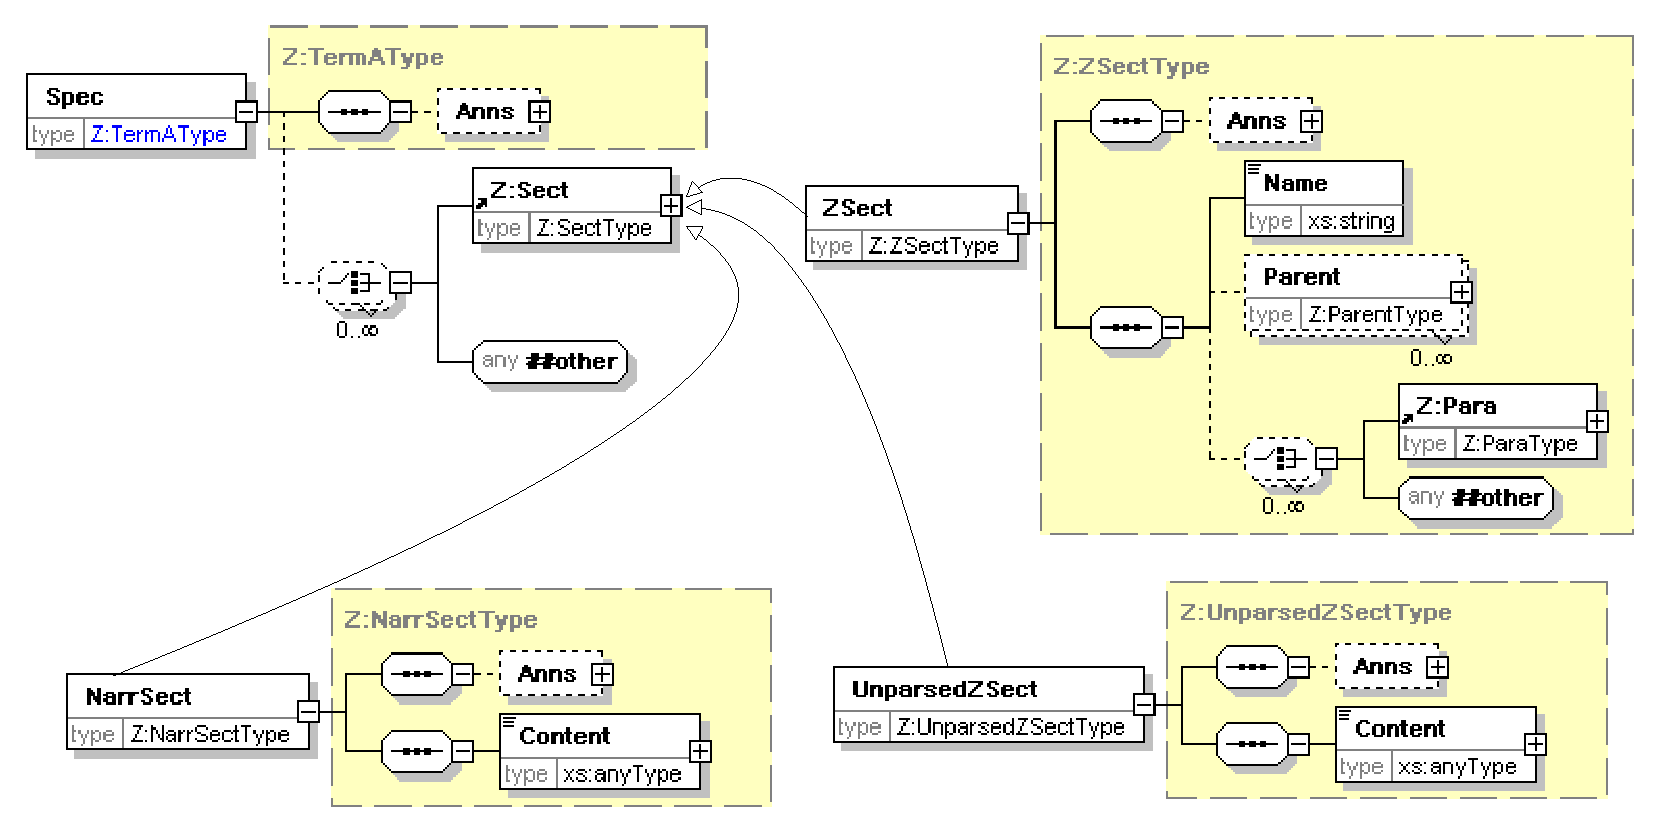
\includegraphics[width=\textwidth]{specall.eps}
  \caption{XML structure for an entire Specification.  The arrows pointing
  towards \AFont{Sect} indicate that 
  \AFont{ZSect}, \AFont{UnparsedZSect} and \AFont{NarrSect} are in the
  \AFont{Sect} substitution group, so each \AFont{Sect} element can be
  replaced by any one of them.} 
  \label{fig:spec}
\end{figure}

Fig.~\ref{fig:spec}
shows a diagrammatic presentation of the corresponding XML
structure, omitting some details such as attributes.
It shows that a specification is a sequence of zero or more constructs,
where each construct is either a parsed section ($\AFont{ZSect}$), 
an unparsed section ($\AFont{UnparsedZSect}$), a narrative portion
($\AFont{NarrSect}$) or some other kind of arbitrary (non Z-related) XML
element (the $\AFont{any\ \#\#other}$).  Each parsed $\AFont{ZSect}$
section must be  
a sequence of an optional set of annotations, then a name, then zero or
more parents, then zero or more paragraphs (or other XML elements).
The top-level \AFont{Spec} element also has three optional attributes 
(not shown) to record its \emph{Creator} and the \emph{Date} and
\emph{Time} of the last modification. 
Note that inside an \AFont{Anns} tag, \emph{any} XML elements are
allowed---our XML proposal pre-defines several annotations,
but other tools are free to define more.  We have set $processing=lax$
within the \AFont{Anns} element, which means that Z tools and other
validation tools should simply ignore any annotations they do not
understand. 

Within a \AFont{ZSect}, the list of parent names need not include
\textit{prelude}, as that is implicitly a parent of all sections.
If there are no parents,
the \AFont{ZSect} element does not record whether or not
the keyword \AFont{parents} occurred in the concrete representation.
This doesn't matter sufficiently to deserve the declaration of an attribute.


\paragraph{Support for Z Extensions.}
There have been numerous extensions of Z in the past, and this will
probably continue.  Furthermore, within a Z specification, we want
to allow complementary kinds of specification, such as CSP specifications,
UML diagrams, or new kinds of paragraphs defined by some extension of Z
like Object-Z or TCOZ.  
Fig.~\ref{fig:spec} shows that, within specifications and sections, our XML
mark-up allows arbitrary elements from \emph{other} namespaces to be
interspersed with Z constructs.  
This means that the XML tags that belong to the standard Z
namespace will be checked and processed by Z tools, while text and unknown
tags (from other namespaces) will be ignored.  In other words, the formal Z
constructs (sections and paragraphs) are viewed as being part of a
larger narrative, which may contain other kinds of 
top-level mark-up.  This is a more permissive, egalitarian style of
mark-up than allowing only standard Z constructs to appear at the top
level.


\subsection{Paragraphs}

Toyn's DTD defined \verb!Z:Para! to be a \emph{choice} between six
kinds of paragraph.  XML Schema gives us several different ways of doing
this, and we have decided to use a newish XML Schema feature,
\emph{Substitution Groups}, rather than choice groups, because substitution
groups are similar to an object-oriented subtyping structure (where a
subtype object can replace a supertype object), and can support inheritance
of attributes and elements.   

Substitution groups make it easy to extend the structure.  For example, a Z
extension can add a new kind of paragraph simply by defining a new
element with \texttt{substitutionGroup="Para"}.  It is also easy to add new
features to one of the subtypes, like \texttt{AxPara}, by declaring a new
element whose type extends or restricts the type of \texttt{AxPara} and
says \texttt{substitutionGroup="AxPara"} (the substitution relationship is
transitive).

Here is the XML Schema definition for \AFont{Para}.
It is declared to be abstract so that XML files \emph{must} contain a
more specific kind of paragraph, wherever a \texttt{Para} element is 
expected.
\begin{verbatim}
<xs:element name="Para" type="ParaType" abstract="true"/>
\end{verbatim}

The following subsections go
through each kind of paragraph, describing their structure.


\subsubsection{Given Types Paragraph}\label{giventypes}

The following table lists the components of a given types paragraph.

\begin{small}
\begin{center}
\begin{tabular}{|l|l|l|l|}
\hline
{\bf Standard Z} & {\bf \CADiZ} & {\bf \Zeta} & {\bf XML}\\
Given types \AParagraph & \AFont{givdef} & \AFont{Item.AxiomaticDef*} & \AFont{Z:GivenPara}\\
\hline
\AFont{seq} \TNAME & \AFont{dec*} & \AFont{Expr.GivenType} & \AFont{Z:DeclName*}\\
\ASignature & & & \AFont{Z:Anns/Z:TypeEnvAnn}\\
\hline
\end{tabular}
\end{center}
\end{small}

In \CADiZ, all declarations
(given types, generic parameters, variables)
share the same \AFont{dec} representation.
This has the advantage of providing a basis for
tracking all references to each declaration.
% For the moment, we're not worrying about
% how to represent that information as annotations.

In \Zeta, a given types paragraph is represented as
an \AFont{Item.AxiomaticDef}s sequence,
in which each \AFont{Item.AxiomaticDef}'s expression
is an \AFont{Expr.GivenType} containing the name of a given type.
This is an instance of a more general approach:
\Zeta\ represents each Z global definition as an \AFont{Item.AxiomaticDef},
using additional kinds of expressions beyond those of Standard Z
to make this possible.
Concretely, a given types paragraph (or a single given type) is not an
expression, and so \Zeta's representation seems a bit forced. 

In XML, a given types paragraph is marked-up using
the \AFont{Z:GivenPara} element, whose type is shown in
Fig.~\ref{fig:givenpara}.  To save space, we do not show the annotation
elements (\AFont{Anns}) in this and future diagrams, because they appear
on virtually all constructs.

\begin{figure}[htb]
  \centering
  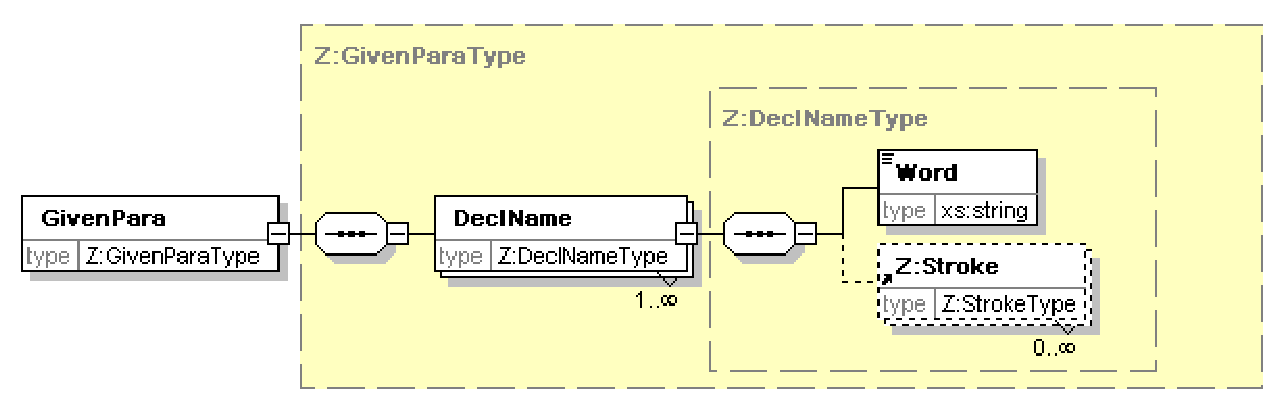
\includegraphics[width=0.8\textwidth]{givenpara.eps}
  \caption{XML structure for Given Type paragraphs}
  \label{fig:givenpara}
\end{figure}


\subsubsection{Axiomatic Description Paragraph}

The following table lists the components of an axiomatic description paragraph.

\begin{small}
\begin{center}
\begin{tabular}{|l|l|l|l|}
\hline
{\bf Standard Z} & {\bf \CADiZ} & {\bf \Zeta} & {\bf XML}\\
(Generic) axdef \AParagraph & \AFont{axidef} & \AFont{Item.AxiomaticDef} & \AFont{Z:AxPara}\\
\hline
\AFont{seq} \TNAME & \AFont{dec*} & \AFont{NameDecl*} & \AFont{Z:DeclName*}\\
\AExpression & \AFont{sch} & \AFont{Expr.Text} & \AFont{Z:SchText}\\
\ASignature & & & \AFont{Z:Anns/Z:TypeEnvAnn}\\
\hline
\end{tabular}
\end{center}
\end{small}

In \CADiZ\ and \Zeta,
non-generic axiomatic description paragraphs are represented
as generic ones with an empty list of generic parameters.
Standard Z differs, as it was thought that the semantics of generics
would be easier to understand if the semantics of non-generics
were defined separately first.

The declarations and predicate parts of an axiomatic description paragraph
are represented differently in the different annotated syntaxes.
Standard Z transforms them to an expression.
\CADiZ\ retains the schema text,
represented by a distinct rule in the annotated syntax.
\Zeta\ views the schema text as an expression.
We believe that some annotations can usefully be placed on schema texts,
and that any single expression appearing where a schema text is expected
is best represented as an inclusion in a schema text,
so that there is somewhere to record those annotations.

Fig.~\ref{fig:axpara} shows our XML structure for the \AFont{AxPara}
element, as well as for schema text and declarations.  Note the
three `subtypes' of \AFont{Decl}.  These are all declared as belonging to
the \AFont{Decl} substitution group so that they can appear wherever
a \AFont{Decl} is required.

The following definitions from the Z standard
(syntactic transformations 12.2.3.1---12.2.3.4)
show how to represent (generic) schema definition paragraphs
and (generic) horizontal definition paragraphs
as (generic) axiomatic description paragraphs.  The $SCH$, $END$ {etc.} are
box tokens, which abstract away from the exact appearances of paragraph
outlines. 
\DTschemadef
\DTgenschemadef
\DThorizdef
\DTgenhorizdef
Generic operator definition paragraphs have their operator names
syntactically transformed to ordinary names
(syntactic transformations 12.2.9.1---12.2.9.4)
and hence they become generic horizontal definition paragraphs
that can be represented as generic axiomatic description paragraphs.

To support resurrection of the original concrete representation, we add an
attribute \AFont{Box} with values: \AFont{OmitBox}, \AFont{AxBox} (the
default), or \AFont{SchBox}.  A further Boolean attribute called
\AFont{Mixfix}, distinguishes whether mixfix syntax is used in the 
definition of a generic operator
e.g. $\_ \rel \_ [X,Y] == \power(X \cross Y)$.

\begin{figure}[!htb]
  \centering
  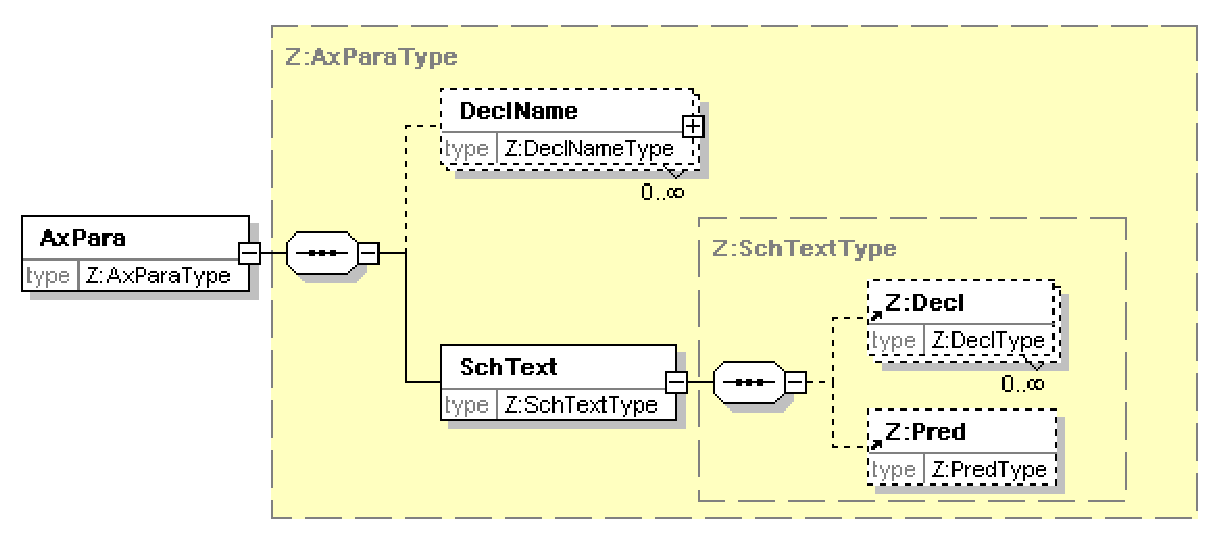
\includegraphics[width=0.8\textwidth]{axpara.eps}
  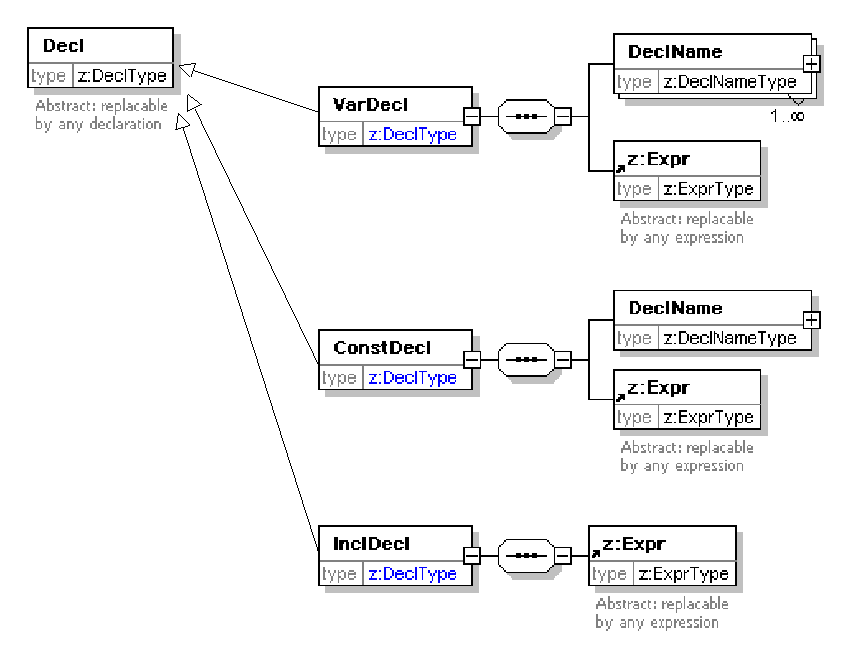
\includegraphics[width=0.6\textwidth]{decls.eps}
  \caption{XML structure for Axiomatic Definition paragraphs, Schema Text
  and Declarations.  The arrows pointing towards \AFont{Decl} indicate that
  \AFont{VarDecl}, \AFont{ConstDecl} and \AFont{InclDecl} are in the
  \AFont{Decl} substitution group, so each \AFont{Decl} element can be
  replaced by any one of them.}
  \label{fig:axpara}
\end{figure}

% \begin{figure}[htb]
%   \centering
%   \caption{XML structure for declarations}
%   \label{fig:decls}
% \end{figure}


\subsubsection{Free Types Paragraph}

The following tables list the components of a free types paragraph.

\begin{small}
\begin{center}
\begin{tabular}{|l|l|l|l|}
\hline
{\bf Standard Z} & {\bf \CADiZ} & {\bf \Zeta} & {\bf XML}\\
Free types \AParagraph & \AFont{datdef} & \AFont{Item.AxiomaticDef*} & \AFont{Z:FreePara}\\
\hline
\AFont{seq} \CFreetype & \AFont{fret+} & \AFont{Expr.FreeType} & \AFont{Z:FreeType+}\\
\ASignature & & & \AFont{Z:Anns/Z:TypeEnvAnn}\\
\hline
\end{tabular}
\end{center}
\end{small}

In \Zeta, the representation of free types paragraphs is similar to that of
other global definitions (see the earlier discussion in the Given Types
section).

\begin{small}
\begin{center}
\begin{tabular}{|l|l|l|l|}
\hline
{\bf Standard Z} & {\bf \CADiZ} & {\bf \Zeta} & {\bf XML}\\
\CFreetype & \AFont{fret} & \AFont{Expr.FreeType} & \AFont{Z:FreeType}\\
\hline
\TNAME & \AFont{dec} & \AFont{NameDecl} & \AFont{Z:DeclName}\\
\AFont{seq} \CBranch & \AFont{bra+} & \AFont{Branch+} & \AFont{Z:Branch+}\\
\hline
\end{tabular}
\end{center}
\end{small}

The representation of a branch is very different in different tools,
and so cannot readily be tabulated.

\begin{small}
\begin{center}
\begin{tabular}{|l|l|}
\hline
{\bf Standard Z} & {\bf XML}\\
\CBranch & \AFont{Z:Branch}\\
\hline
$\TNAME$ & \AFont{Z:DeclName}\\
\AExpression & \AFont{Z:Expr?}\\
\hline
\end{tabular}
\end{center}
\end{small}

In \CADiZ, a \AFont{Branch}'s name and optional expression
are both represented by a single \AFont{dec} value,
allowing references to the name to be tracked.

In \Zeta, a \AFont{Branch} is either a \AFont{Constant} or a \AFont{Function}.
A \AFont{Constant} has just a \AFont{NameDecl},
whereas a \AFont{Function} has both a \AFont{NameDecl} and an \AFont{Expr}.

In XML, a free types paragraph is marked-up using
the \AFont{Z:FreePara} element, whose type is shown in Fig.~\ref{fig:freepara}.

\begin{figure}[htb]
  \centering
  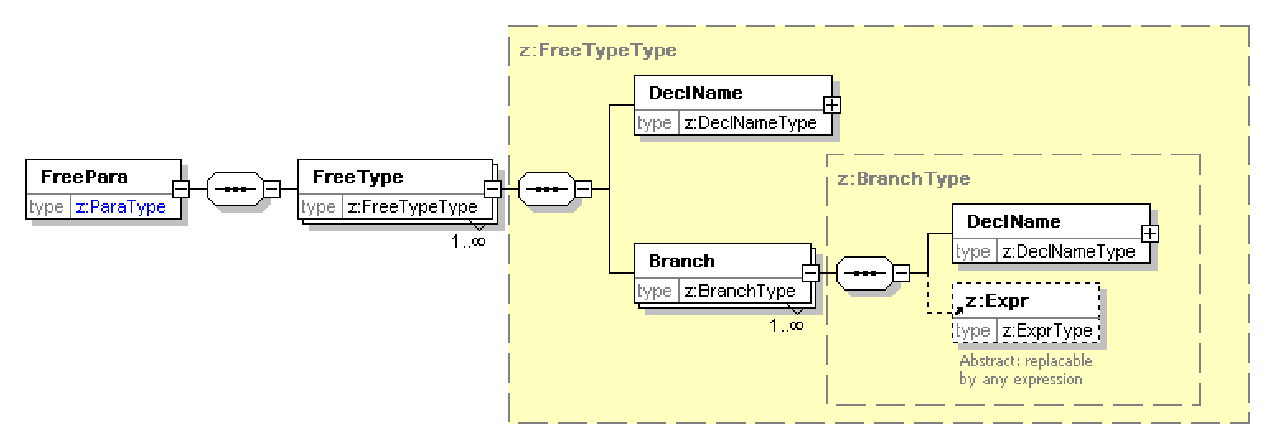
\includegraphics[width=\textwidth]{freepara.eps}
  \caption{XML structure for Free Type paragraphs}
  \label{fig:freepara}
\end{figure}


\subsubsection{Conjecture Paragraph}

Standard Z conjectures have a single consequent predicate and zero or more
generic parameters. 

\Zeta\ does not support conjecture paragraphs.

In \CADiZ, conjectures are represented as particular cases of
a more general syntax for sequents.
Sequents allow for zero-or-more generic parameters,
zero-or-more levels of nested \AFont{DeclPart}s,
zero-or-more antecedent predicates,
zero-or-more consequent predicates,
and a name for the sequent.
This more general syntax assists humans doing proofs interactively,
but adds nothing semantically: any sequent can be rearranged
into an equivalent single-consequent form that conforms to the Z standard
(ignoring the sequent's name, which can be thought of as an annotation).
Other reasoning tools for Z may use different representations for sequents.
So it seems inappropriate to define an XML mark-up for anything
more complicated than a Standard Z (generic) conjecture.

The following table lists the components of a conjecture paragraph.

\begin{small}
\begin{center}
\begin{tabular}{|l|l|}
\hline
{\bf Standard Z} & {\bf XML}\\
(Generic) conjecture \AParagraph & \AFont{Z:ConjPara}\\
\hline
\AFont{seq} \TNAME & \AFont{Z:DeclName*}\\
\APredicate & \AFont{Z:Pred}\\
\ASignature & \AFont{Z:Anns/Z:TypeEnvAnn}\\
\hline
\end{tabular}
\end{center}
\end{small}

In XML, a conjecture paragraph is marked-up using
the \AFont{Z:ConjPara} element (Fig.~\ref{fig:conjpara}).
This representation suffices for both generic and non-generic
conjecture paragraphs: the sequence of generic parameters is empty in the
non-generic case. 

\begin{figure}[htb]
  \centering
  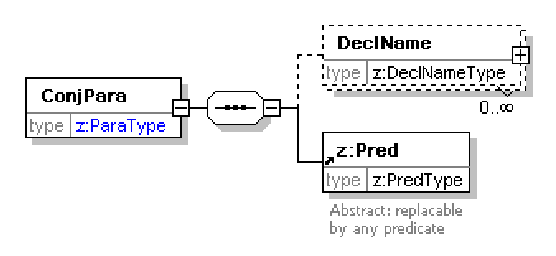
\includegraphics[width=0.6\textwidth]{conjpara.eps}
  \caption{XML structure for Conjecture paragraphs}
  \label{fig:conjpara}
\end{figure}


\subsubsection{Operator Template Paragraph}

Standard Z has operator template paragraphs in its concrete syntax
but not in its annotated syntax,
because they affect how the specification is parsed
but have no further meaning themselves.
To be able to interchange them and resurrect their concrete syntax,
and the concrete syntax of the operators they define,
the XML mark-up must provide a representation of them.

Operator templates are one of the innovations of Standard Z
and were subject to some late changes,
so tools are unlikely to support operator templates exactly as in Standard Z
(excepting \CADiZ).
The concrete syntax allows explicit declaration of precedence and associativity
only for infix function and infix generic operators.
Other operators have implicit precedences and associativities,
which it is convenient to make explicit in the annotated syntax.

The following table lists the components of an operator template paragraph.

\begin{small}
\begin{center}
\begin{tabular}{|l|l|l|l|}
\hline
{\bf Standard Z} & {\bf \CADiZ} & {\bf \Zeta} & {\bf XML}\\
Operator template \AParagraph & \AFont{fixdef} & \AFont{Fixity} & \AFont{Z:OptempPara}\\
\hline
\AFont{Category} & \AFont{cat} & \AFont{isGeneric} & \AFont{Z:Cat (Attr)}\\
\CPrec & \AFont{nat} & \AFont{prio} & \AFont{Z:Prec (Attr)}\\
\CAssoc & \AFont{boole} & \AFont{?} & \AFont{Z:Assoc (Attr)}\\
\AFont{Template} & \AFont{(nat,word)+} & \AFont{Component*} & See Fig.~\ref{fig:optemppara}\\
\hline
\end{tabular}
\end{center}
\end{small}

In \CADiZ, a \AFont{Template} is represented as a list of pairs.
While this enforces alternation of operators and operands,
it may unfortunately appear to add an unwanted operand at the beginning
and/or an unwanted operator at the end,
for which distinguishable values are needed to avoid confusion.

In \Zeta, a \AFont{Template} is represented as a list of \AFont{Component}s.
Each \AFont{Component} is either a \AFont{Keyword}, \AFont{Operand} or
\AFont{OperandList}.
\Zeta\ appears to parse declarations of associativity,
but it does not appear to keep a representation of associativity
in its annotated syntax.
Its annotated syntax also appears not to distinguish
relation and function categories.

In XML, an operator template paragraph is marked-up using
the \AFont{Z:OptempPara} element (Fig.~\ref{fig:optemppara}).
In addition, each \AFont{Z:OptempPara} has three attributes:
\begin{description}
\item[\AFont{Cat}] (category) which can equal \AFont{Relation},
  \AFont{Function} or \AFont{Generic}.  
\item[\AFont{Assoc}] which can be \AFont{Left} or \AFont{Right}. 
\item[\AFont{Prec}] (precedence) which is a natural number.
\end{description}

\begin{figure}[htb]
  \centering
  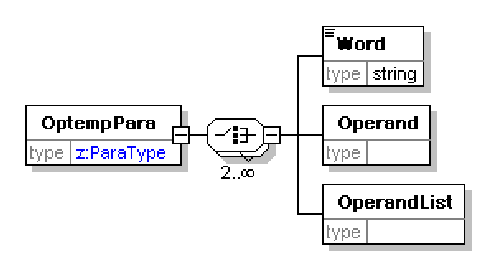
\includegraphics[width=0.5\textwidth]{optemppara.eps}
  \caption{XML structure for Operator Template paragraphs}
  \label{fig:optemppara}
\end{figure}


\subsubsection{Narrative Paragraph}

To allow natural language narrative to appear between Z paragraphs,
we define a \AFont{NarrPara} element, containing annotations
and a \AFont{Contents} element which contains arbitrary unicode and
markup.  This is similar to \AFont{NarrSect} in Fig.~\ref{fig:spec}.

\subsubsection{Unparsed Paragraph}

Our final kind of paragraph does not appear in {\Zeta}
or the Z standard, because their annotated syntax representations
are used only \emph{after} an entire specification has been successfully
parsed.  However, since our XML format may be our source representation,
we need to be able to represent erroneous (unparsable) specifications as
well.  Similar to the \AFont{ErrorDef} paragraph in \CADiZ, we use a
special paragraph called \AFont{UnparsedPara}, whose structure is the
same as \AFont{UnparsedZSect} (see Fig.\ref{fig:spec}).
If a tool attempts to parse an \AFont{UnparsedPara}, it may return a parse
error, or one or more paragraphs (which will replace the
\AFont{UnparsedPara}).  Similarly, at the top level of a specification, an
\AFont{UnparsedZSect} may become one or more sections if it can be parsed.

% \begin{figure}[htb]
%   \centering
%   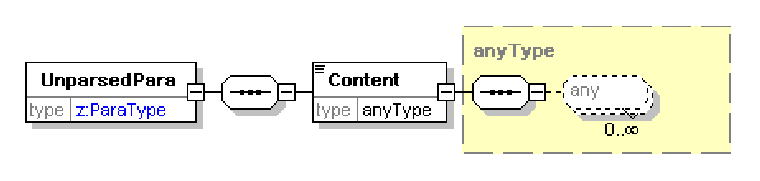
\includegraphics[width=0.5\textwidth]{unparsedpara.eps}
%   \caption{XML structure for Unparsed paragraphs}
%   \label{fig:unparsed}
% \end{figure}


\subsection{Predicates and Expressions} \label{sec:expr}

We shall not go into details about the structure of predicates and
expressions etc., but will discuss some specific features and give
a few short XML examples to give the flavour of our approach.

As for paragraphs, declarations and strokes, we define \AFont{Expr}
and \AFont{Pred} to be abstract elements, and use substitution
groups to allow specific concrete kinds of expressions and predicates to be
used in their place.  To capture the commonalities between various 
kinds of expressions, we define a hierarchy of XML types
(Fig.~\ref{fig:hier}).   We expect that this same hierarchy can be
used in Z tools that are written in object-oriented languages.
Then the various concrete predicate and
expression elements are defined as members of these types, as the
following examples illustrate (\verb!grp! stands for
\verb!substitutionGroup!):
\begin{small}
\begin{verbatim}
<element name="OrPred"      type="Z:Pred2Type"    grp="Z:Pred"/>
<element name="ImpliesPred" type="Z:Pred2Type"    grp="Z:Pred"/>
<element name="ForallPred"  type="Z:QntPredType"  grp="Z:Pred"/>
<element name="ExistsPred"  type="Z:QntPredType"  grp="Z:Pred"/>
<element name="FalsePred"   type="Z:FactType"     grp="Z:Pred"/>
<element name="TruePred"    type="Z:FactType"     grp="Z:Pred"/>

<element name="LambdaExpr"  type="Z:Qnt1ExprType" grp="Z:Expr"/>
<element name="MuExpr"      type="Z:QntExprType"  grp="Z:Expr"/>
<element name="LetExpr"     type="Z:Qnt1ExprType" grp="Z:Expr"/>
<element name="SetCompExpr" type="Z:QntExprType"  grp="Z:Expr"/>
\end{verbatim}
\end{small}

Some expressions and predicates have special features to enable the
concrete syntax to be resurrected.  Z has several
conjunction operators ($\land$, $;$, newline and the implicit conjunctions
within $a < b < c$), which are all represented by the \AFont{AndPred}
element (of type \AFont{Pred2Type}) with an attribute to record which
kind of conjunction it came from.  The \AFont{RefExpr}, \AFont{ApplExpr}
and \AFont{MemPred} elements have a Boolean attribute called \AFont{Mixfix}
to record whether the application uses mixfix notation or not.


\newcommand{\I}{\hbox{\ \qquad}}
\begin{figure}[htb]
\begin{scriptsize}
\begin{tabular}{ll}
TermType                  &supertype of all Z constructs \\
\I StrokeType             &supertype of the 4 kinds of name decorations\\
\I AnnType                &supertype of all annotations\\
\I TermAType              &supertype of all annotatable constructs\\
\I\I  Spec                &\\
\I\I  SectType            &supertype of all section types \\
\I\I\I  ZSectType         &\\
\I\I\I  UnparsedZSectType &\\
\I\I\I  NarrSectType      &\\
\I\I  ParaType            &supertype of all paragraph types\\
\I\I\I  GivenParaType\\
\I\I\I  AxParaType\\
\I\I\I  FreeParaType\\
\I\I\I  ConjParaType\\
\I\I\I  OptempParaType\\
\I\I\I  UnparsedParaType\\
\I\I  DeclType            &supertype of all declarations\\
\I\I\I  VarDecl\\
\I\I\I  ConstDecl\\
\I\I\I  InclDecl\\
\I\I  PredType\\
\I\I\I  Pred2Type         &supertype of all binary predicates\\
\I\I\I  QntPredType       &supertype of all quantifier predicates\\
\I\I\I  FactPredType      &supertype of the true/false predicates\\
\I\I  ExprType\\
\I\I\I  Expr1Type         &supertype of all unary expressions\\
\I\I\I  Expr2Type         &supertype of all binary expressions\\
\I\I\I\I  LogExprType     &supertype of all binary schema operators\\
\I\I\I  QntExprType       &supertype of all quantifier exprs\\
\I\I\I\I  Qnt1ExprType    &supertype of quantifier exprs with compulsory body\\
\I\I\I\I\I  ExistsExprType &supertype of existential schema exprs\\
\I\I\I  Expr0NType        &supertype of exprs with 0 or more subexprs\\
\I\I\I\I  Expr2NType      &supertype of exprs with 2 or more subexprs\\
\I\I  TypeType            &supertype of all Z base types used in annotations\\
\I\I  ParentType          &\\
\I\I  FreeTypeType        &\\
\I\I  BranchType          &\\
\I\I  SchTextType         &\\
\I\I  NameType            &\\
\end{tabular}
\end{scriptsize}
\caption{The hierarchy of XML complex types in ZML.}
\label{fig:hier}
\end{figure}


\paragraph{The Challenge of Nested Identical Names.}

In Z it is quite common to have several levels of declarations nested 
inside one another.  If two levels declare the same name $X$, then
expressions inside the inner's scope cannot normally refer to the outer $X$.
However, there are situations like the following example, where the
instantiation of generic operators during type checking must
introduce references to the outer $X$ (the $\# \{a\}$ becomes
$\#[X]\{a\}$). This creates a problem, because naively introducing
$X$ at this point causes it to bind to the inner $X$ rather than 
the outer $X$. 
\begin{zed}
    [X] \\
\end{zed}
\begin{axdef}
    a : X
\where
    \exists X : \nat @ \# \{a\} = X
\end{axdef}

% Or: \forall X : \power \arithmos @ X = \{a\}
%     The abstract syntax for the relational predicate is
%     (X, \{a\}) \in (\_ = \_)[\power X]

None of the previous DTD or XML Schema proposals solve this problem.  The
traditional solution is to rename the bound $X$.  But to allow exact
resurrection of concrete syntax we do \emph{not} want to rename bound
variables.  The Z standard solves this problem by creating suit-decorated
synonyms of type names (e.g., $X\heartsuit$) and making implicit
instantiations refer to those synonyms.  We want a
more general solution than this, so that tools can perform a variety of
transformations, then produce correct XML using the original names, even
though the scopes of those names may have changed.

\CADiZ\ solves this problem by using references
to link each name to a corresponding declaration.
We do the same thing in XML, by using the ID and IDREF
cross-reference features of XML to allow a variable reference to point to
a specific variable declaration (which may not be the nearest nested
name).  Declarations of names may have an ID-valued attribute called
$\AFont{Id}$, while references to names may have an IDREF-valued attribute
called $\AFont{Decl}$ which links to a declaration.  Since soundness relies
on following these references correctly, 
every Z tool must be capable of following them, and pretty printers must
display the output unambiguously (either by renaming one of the bound
variables, or by making the generic instantiations implicit again to hide
the problem reference).  
% Ian notes: Making generic instantiations implicit again sounds dangerous,
%     though if the expression denotes a carrier set then I guess it
%     must be safe.

The full mark-up of the above example is shown in Appendix A.
The XML for the declaration of the global name $X$ is:
\begin{small}
\begin{verbatim}
<GivenPara><DeclName Id="X.3"><Word>X</Word></DeclName></GivenPara>
\end{verbatim}
\end{small}
while an expression that references this $X$ can be marked up as:
\begin{small}
\begin{verbatim}
<RefExpr><RefName Decl="X.3"><Word>X</Word></RefName></RefExpr>
\end{verbatim}
\end{small}

%% NOTE: The following idea was dropped, for several reasons.
%%    1. declaration becomes unparsed, while references to it stay parsed.
%%    2. In (\forall S @ x=3) the x will presumably point to the S, 
%%       but this does not uniquely determine the text of the name x.
%%
% Note that in variable references that contain an ID
% value, the actual name of the variable is redundant, since it can be
% obtained from the declaration.  For this reason, we decided to simplify
% \AFont{RefExpr} so that it always contains an ID attribute, rather than
% the word and decorations of the name.  That is, rather than writing
% \begin{verbatim}
%     <RefExpr><RefName><Word>name</Word><InStroke></RefName></RefExpr>
% \end{verbatim}
% to refer to the variable $name?$, we write just
% \begin{verbatim}
%     <RefExpr Decl="name?.3"></RefExpr>,  or
%     <RefExpr Decl="name?.3"/>,
% \end{verbatim}
% where the declaration of $name?$ contains the attribute
% \verb!Id="name?.3"!.  Note that human readability can be retained
% by using the variable name as a prefix of the ID label, as illustrated here.

% \begin{figure}[htb]
%   \centering
%   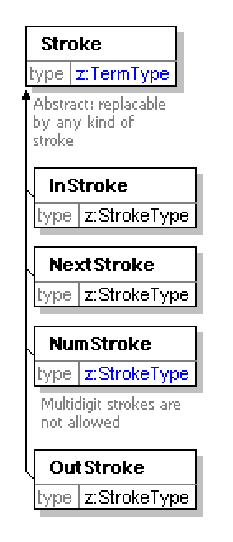
\includegraphics{stroke.eps}
%   \caption{XML structure for decorations (strokes) on names}
%   \label{fig:stroke}
% \end{figure}


\section{Conclusions}

We have defined an XML mark-up format for standard Z, based on
combining the best features from the standard and several existing 
tools.  The XML Schema has been validated, and several small examples
have been validated against the schema.  We are now seeking feedback 
and comments on the design, particularly on the following issues:
\begin{enumerate}
\item Two alternative approaches to annotations: the approach taken
  here is for each term to have an optional \AFont{Anns} slot that can
  contain arbitrary XML (which is not validated or checked in any way).  
  An alternative approach would be to put new kinds of annotations into
  separate documents (with their own XML Schema) and use IDREF links
  to link each annotation to the appropriate Z term (which would have an ID
  attribute).
\item Two alternative approaches to narrative and non-standard portions of
  Z specification documents.  Should narrative paragraphs and non-Z XML
  mark-up be viewed as subordinate to the Z, or should it be mixed in
  with the Z constructs on an equal basis (as in this paper)?  The former
  approach allows stricter XML validation of the document, because every
  top-level paragraph is of a known type and can be checked (except that
  \AFont{Narrative} paragraphs would be allowed arbitrary contents).
  The latter approach (which we have taken) makes it easy to add new kinds
  of paragraphs 
  (e.g., for Z extensions), even without extending the XML Schema, but
  means that standard Z tools will quietly ignore all unknown kinds of
  paragraphs.
\item Unparsed fragments.  Is it really useful to be able to have some
  paragraphs or sections unparsed?  Would an even finer granularity be
  useful (\AFont{Expr} and \AFont{Pred} etc.)?  Or should we disallow
  unparsed portions and insist that this XML mark-up be used only for
  syntactically correct specifications? 
\item Mathematical Symbols.  We expect that the special symbols used in Z
  will normally be represented in XML documents using their binary Unicode
  representation (e.g., UTF8).  However, this means that the documents are
  not ASCII-based and are only human-readable if you have a full Unicode
  font.  Would it be useful to define symbolic names for all the Z symbols
  (this can be done using DTD entities, or XML Schema elements with fixed
  contents) so that the Z specifications can be pure ASCII?  Or will this
  be irrelevant once full Unicode fonts and Unicode editors become widely
  available? 
\end{enumerate}

Combining the best features from the Z standard and several existing
tools has been worthwhile,
as can be seen by considering the main influences on the XML structure.
The \texttt{Specification} representation is influenced mainly by the form
of XML. 
The \texttt{Section} representation is influenced mainly by \Zeta.
The \texttt{Paragraph} representation is influenced mainly by Standard Z,
with the commonality between generics and non-generics taken from
both \CADiZ\ and \Zeta,
and the template representation in operator templates taken from \Zeta.
The \texttt{Predicate} representation is influenced mainly by \CADiZ\ and
\Zeta, which use remarkably similar representations.
The \texttt{Expression} representation falls between those of \CADiZ\ and
\Zeta.  The representations of schema text and names 
are influenced mainly by \Zeta.

Next we plan to derive a set of open-source Java classes from this XML
schema, preferably by using either JAXB\footnote{See
  \url{http://java.sun.com/xml/jaxb}.} or XSLT to 
transform the schema into Java source. 
These Java classes will support the visitor design
pattern~\cite{gamma:design-patts95}, so that functionality such as type
checkers, 
transformation tools, simplifiers and pretty printers can easily be written
as add-on packages.  This will dramatically reduce the usual initial
barriers of creating new Z tools (parsing, type-checking etc.) and make it
easier for student projects and other researchers to experiment with
building new Z tools.

Another important step is for existing Z tools to support this
XML format, by adding import and export functions that read and write it.
{\CADiZ} already exports an XML format that is close to this one.

\begin{small}
\bibliographystyle{plain}
\bibliography{cmp}
\end{small}

\newpage
\appendix
\section{XML Mark-Up of Example from Sect.~\ref{sec:expr}}
\newcommand{\NAT}{$\nat$}
\newcommand{\EXISTS}{$\exists$}
\begin{small}
\begin{alltt}
  <NarrPara>
    <Content>First we declare X to be a given set.</Content>
  </NarrPara>
  <GivenPara>
    <DeclName Id="X.3"> <Word>X</Word> </DeclName>
  </GivenPara>

  <NarrPara>
    <Content>This axiomatic definition declares a:X, with the
    constraint: (\EXISTS X:\NAT @ #\{a\} = X)</Content>
  <NarrPara>
  <AxPara>
    <SchText>
      <VarDecl>
        <DeclName> <Word>a</Word> </DeclName>
        <RefExpr><RefName><Word>X</Word></RefName></RefExpr>
      </VarDecl>

      <ExistsPred>
        <SchText>
          <VarDecl>
            <DeclName> <Word>X</Word> </DeclName>
            <RefExpr><RefName><Word>\NAT</Word></RefName></RefExpr>
          </VarDecl>
        </SchText>
        <MemPred>
          <TupleExpr>
            <ApplExpr>
              <RefExpr>
                <RefName><Word>#</Word></RefName>
                <RefExpr>
                  <RefName Decl="X.3"> <Word>X</Word>
                  </RefName>
                </RefExpr>
              </RefExpr>
              <SetExpr>
                <RefExpr><RefName><Word>a</Word></RefName></RefExpr>
              </SetExpr>
            </ApplExpr>
            <NumExpr Value="1"/>
          </TupleExpr>
          <RefExpr><RefName><Word>=</Word></RefName></RefExpr>
        </MemPred>
      </ExistsPred>
    </SchText>
  </AxPara>
\end{alltt}
\end{small}
\end{document}
